 \documentclass{beamer}

\usetheme{MagdeburgFIN}
\usefonttheme{structurebold}
\usepackage{graphicx}
\usepackage{wrapfig,lipsum}
\usepackage{float}
\usepackage{url}
\usepackage{pdfpages}
\usepackage[ngerman]{babel}
\usepackage[utf8]{inputenc}

\title{Thread Pool in GeckoDB/BOLSTER}
\subtitle{Milestone IV: Final presentation (wrap-up + evaluation results) }
\author{Johann Wagner, Johannes Wünsche, Marten Wallewein-Eising, Robert Jenderise}
\date{\today}
\institute{Otto von Guericke University, Magdeburg}

\begin{document}

\begin{frame}[plain]
 \titlepage
\end{frame}

\section[Agenda]{}
	\begin{frame}
	\frametitle{Agenda}
	\tableofcontents
	\end{frame}

\section{Previously...}
\begin{frame}
	\begin{center}
		\huge Previously...
	\end{center}
\end{frame}

\begin{frame}
	\frametitle{Previously on Thread Pool in GeckoDB/BOLSTER}
	\begin{center}
		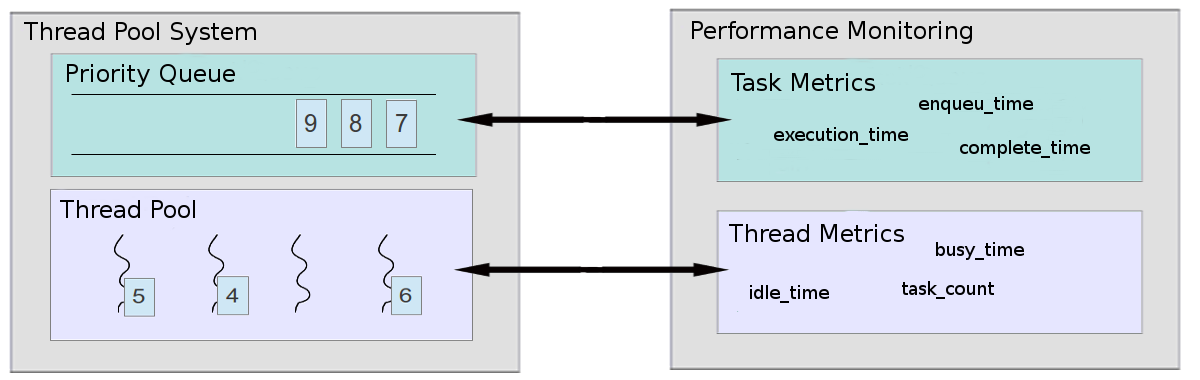
\includegraphics[width=0.9\textwidth]{img/pool_structure.png}
	\end{center}
	\begin{center}
		Thread Pool System
	\end{center}
\end{frame}

\begin{frame}
	\frametitle{Previously on Thread Pool in GeckoDB/BOLSTER}
	\begin{center}
		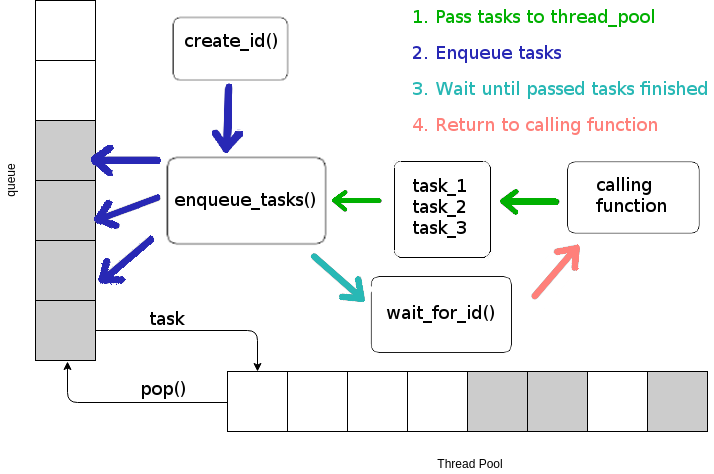
\includegraphics[width=0.8\textwidth]{img/pool_queue.png}
	\end{center}
	\begin{center}
		Enqueuing and Waiting for Tasks
	\end{center}
\end{frame}

\begin{frame}
	\frametitle{Previously on Thread Pool in GeckoDB/BOLSTER}
	\begin{center}
		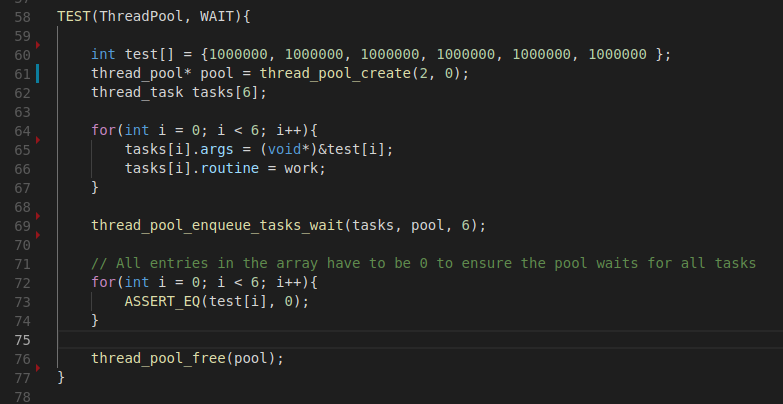
\includegraphics[width=0.9\textwidth]{img/thread_pool_use.png}
		
	\end{center}
	\begin{center}
		Thread Pool Usage
	\end{center}
\end{frame}

\section{Optimizations}
\begin{frame}
\begin{center}
	\huge Optimizations
\end{center}
\end{frame}

\begin{frame}
	\frametitle{wait slot distribution}
	\begin{center}
	
	\begin{columns}
		\begin{column}{0.28\textwidth}
			linear search from the beginning:	
		\end{column}
		\begin{column}{0.7\textwidth}
			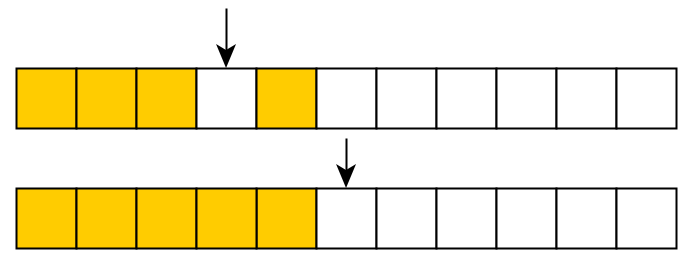
\includegraphics[width=1.0\textwidth]{img/slot_compact.png}
		\end{column}
	\end{columns}
	\begin{columns}
		\begin{column}{0.28\textwidth}
			distribute over cache lines:
		\end{column}
		\begin{column}{0.7\textwidth}
			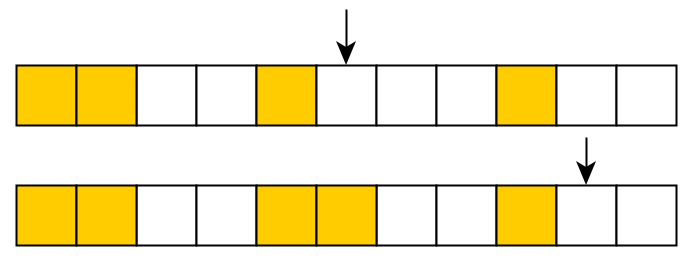
\includegraphics[width=1.0\textwidth]{img/slot_distributed.png}
		\end{column}
	\end{columns}
	\end{center}
\end{frame}

\begin{frame}
	\frametitle{priority queue}
	\begin{itemize}
		\item binary heap with a single array
		\item fast insertion, extraction of the smallest element
		\item all operations require full access to the array: poor concurrency
		\item state of the art: skip list with logical operations and delayed deletes
	\end{itemize}
	\begin{center}
		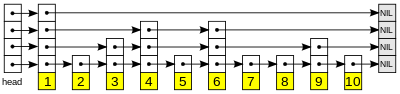
\includegraphics[width=0.7\textwidth]{img/skip_list.png}
	\end{center}
\end{frame}

\section{Evaluation}
\begin{frame}
	\begin{center}
		\huge Evaluation
	\end{center}
\end{frame}

\begin{frame}
	\frametitle{Evaluation Setup}
	\begin{itemize}
		\item Tests run on different environments, including Windows 10, MacOS High Sierra and Archlinux
		\item Presentation results measured on Archlinux with kernel 4.17.2-1 and 24 GB DDR4-SODIMM
		\item Each measure was repeated 3 times and an average value is used
	\end{itemize}
\end{frame}

\begin{frame}
	\frametitle{Evaluation Benchmarks}
	\begin{itemize}
		\item Compare against approximated implementation of BOLSTER (baseline)
		\item Evaluation of waiting time for different thread pool sizes
		\item Utilization of different slot distribution strategies
		\item Utilization of lock-free vs mutex based heap
	\end{itemize}
\end{frame}

\begin{frame}
	\frametitle{Comparison against Baseline Implementation}
	\begin{center}
		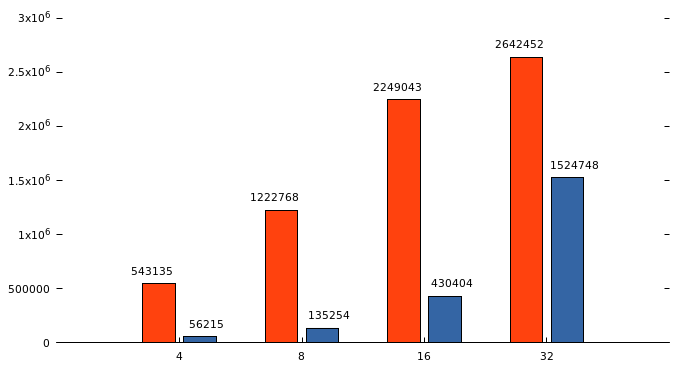
\includegraphics[width=0.8\textwidth]{img/pool_baseline.png}
	\end{center}
	
\end{frame}

\begin{frame}
	\frametitle{Waiting Time Evaluation}
	\begin{center}
		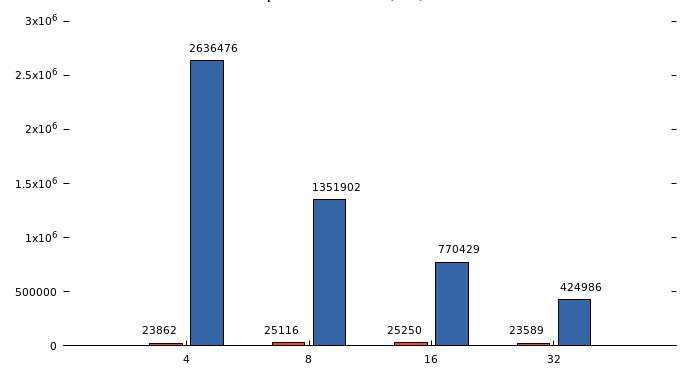
\includegraphics[width=0.8\textwidth]{img/pool_avg.png}
	\end{center}

\end{frame}

\begin{frame}
	\frametitle{Utilization of different slot distribution strategies}
	\begin{columns}
		\begin{column}{0.74\textwidth}
			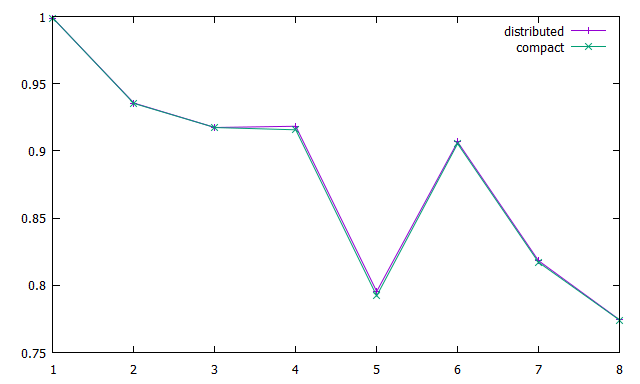
\includegraphics[width=1.0\textwidth]{img/slot_distr.png}
		\end{column}
		\begin{column}{0.26\textwidth}
			\begin{itemize}
				\item[$\Rightarrow$] small impact on performance
				\item[$\Rightarrow$] no visible scaling with \#threads
			\end{itemize}
		\end{column}
	\end{columns}
\end{frame}

\begin{frame}
	\frametitle{Utilization of lock-free vs mutex based priority queue}
	\begin{columns}
		\begin{column}{0.76\textwidth}
			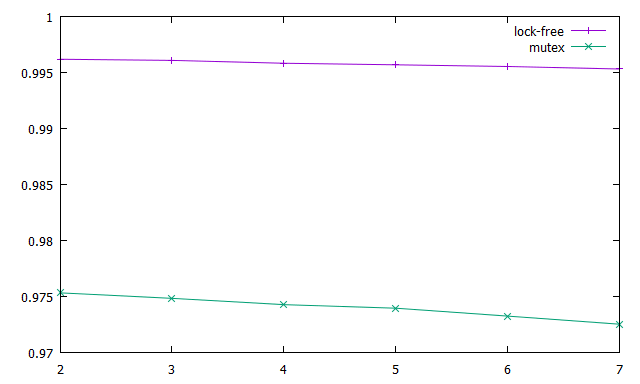
\includegraphics[width=1.0\textwidth]{img/lock_free.png}
		\end{column}
		\begin{column}{0.24\textwidth}
			\begin{itemize}
				\item[$\Rightarrow$] reduced constant overhead
				\item[$\Rightarrow$] better asymptotic behaviour
			\end{itemize}
		\end{column}
	\end{columns}
\end{frame}

\section{Summary}
\begin{frame}
	\begin{center}
		\huge Summary
	\end{center}
\end{frame}

\begin{frame}
	\frametitle{Summary}
	\textbf{Evaluation results:}
	\begin{itemize}
		\item Better execution performance as baseline implementation
		\item Constant average waiting time over different pool sizes
		\item Small performance costs for enqueueing and waiting
	\end{itemize}
\end{frame}

\begin{frame}
\frametitle{Summary}
	\textbf{Project Evaluation:}
	\begin{itemize}
		\item All requirements of the thread pool fulfilled
		\item Compact but appropriate implementation feedback
		\item Literature research problematic 
		\begin{itemize}
			\item Few paper about thread pool implementations
			\item Focus on resizing
		\end{itemize}
	\end{itemize}
\end{frame}

%\section{Conclusion}
%	\begin{frame}
%	\begin{center}
%		\huge Conclusion
%	\end{center}
%\end{frame}



\begin{frame}
    \frametitle{Thank you for your attention!}
 	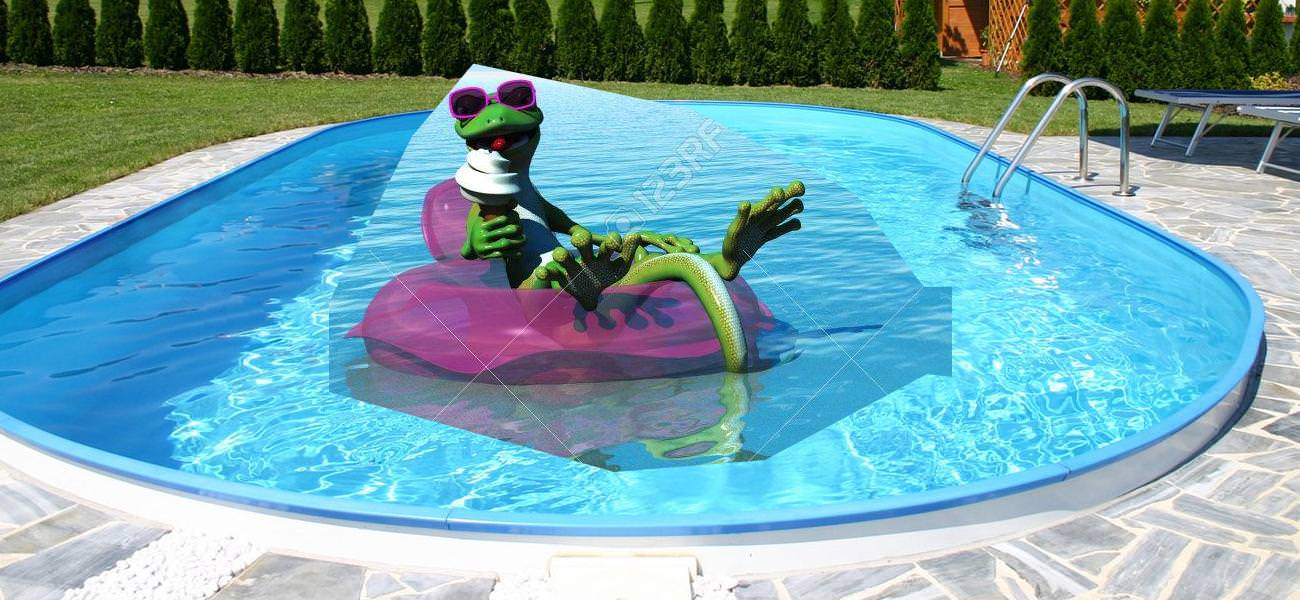
\includegraphics[width=\textwidth]{img/important.jpg}
\end{frame}

\end{document}
